\documentclass[crop,tikz]{standalone}% 'crop' is the default for v1.0, before it was 'preview'
%\usetikzlibrary{...}% tikz package already loaded by 'tikz' option

\usetikzlibrary{arrows,positioning} 
\usetikzlibrary{shapes,decorations}
\usetikzlibrary{calc}
\usetikzlibrary{fit}
\usetikzlibrary{decorations.pathreplacing}
\usetikzlibrary{backgrounds}


\renewcommand{\familydefault}{\sfdefault}


\definecolor{blind_red}{HTML}{D7191C}
\definecolor{blind_orange}{HTML}{FDAE61}
\definecolor{blind_yellow}{HTML}{FFFFBF}
\definecolor{blind_blue}{HTML}{ABD9E9}
\definecolor{blind_blue2}{HTML}{2C7BB6}



\begin{document}
	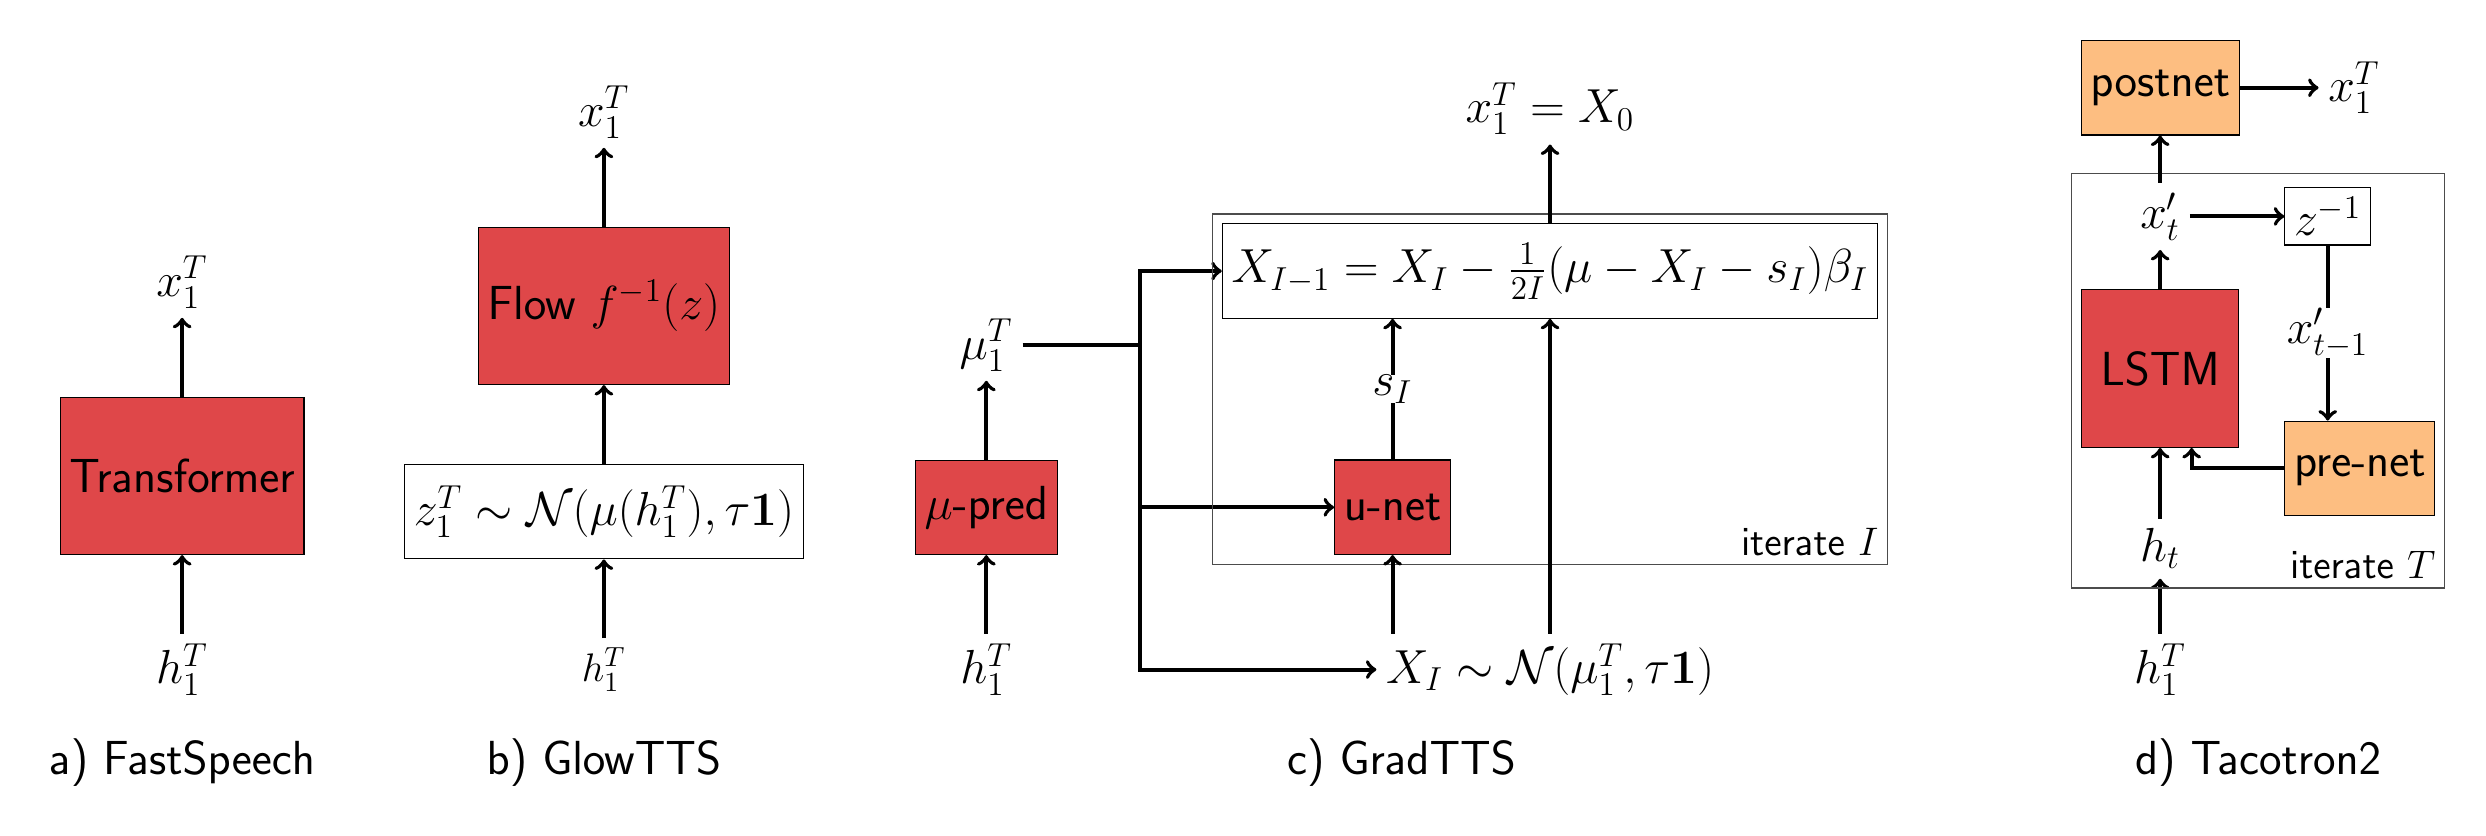
\begin{tikzpicture}[
	    auto,
	    background rectangle/.style={fill=white}, show background rectangle,
	    onlytext/.style={align=center, font=\LARGE},
        halfbox/.style={rectangle, font=\LARGE, minimum size=1.20cm, draw},
	    box/.style={rectangle, font=\LARGE, minimum size=2.00cm, draw},
	    halforangebox/.style={halfbox, fill=blind_orange!80},
	    orangebox/.style={box, fill=blind_orange!80},
	    redbox/.style={box, fill=blind_red!80},
	    normalline/.style={->, line width=0.5mm},
	    state/.style={rectangle, draw, minimum height=0.8cm, minimum width=0.2cm},
	]
	\node[onlytext] (narin) at (0, 0) {$h_1^T$};
	\node[redbox, above=1cm of narin] (nardecoder) {Transformer};
	\node[onlytext, above=1cm of nardecoder] (narout) {$x_1^T$};
	\draw [normalline] (narin) -- (nardecoder);
	\draw [normalline] (nardecoder) -- (narout);

	\node[onlytext, below=0.3cm of narin] (narlabel) {a) FastSpeech};

    % ------------ Flow

    \node[onlytext, right=4.5cm of narin, font=\Large] (flowin) {$h_1^T$};
	\node[halfbox, align=center, above=1cm of flowin] (flowsamp) {$z_1^T \sim \mathcal{N}(\mu(h_1^T), \tau\mathbf{1})$};
	\node[redbox, above=1cm of flowsamp] (flowdecoder) {Flow $f^{-1}(z)$};
	\node[onlytext, above=1cm of flowdecoder] (arout) {$x_1^T$};

	\draw [normalline] (flowin) -- (flowsamp);
	\draw [normalline] (flowsamp) -- (flowdecoder);
	\draw [normalline] (flowdecoder) -- (arout);

	\path let \p1 = (narlabel), \p2 = (flowdecoder) in node [onlytext] (glowlabel) at (\x2,\y1) {b) GlowTTS};

	% ------------ Diffusion

	\node[onlytext, right=4.0cm of flowin] (gradin) {$h_1^T$};
	\node[halfbox, fill=blind_red!80, above=1cm of gradin] (mupred) {$\mu$-pred};
	\node[onlytext, above=1cm of mupred] (mu) {$\mu_1^T$};
	\node[onlytext, right=4.5cm of gradin] (diffsamp) {$X_I \sim \mathcal{N}(\mu_1^T, \tau\mathbf{1})$};

    \draw [normalline] (gradin) -- (mupred);
    \draw [normalline] (mupred) -- (mu);


	\node[halfbox, fill=blind_red!80, align=center, above=1cm of diffsamp, xshift=-2.0cm] (unet) {u-net};


    \path let \p1 = (mu.east), \p2 = ([xshift=-3.0cm]diffsamp.west) in [normalline, draw] (mu.east) -- (\x2, \y1) -- (\x2,\y2) -- (diffsamp.west);
    \path let \p1 = ([xshift=-3.0cm]diffsamp.west), \p2 = (unet.west) in [normalline, draw] (\x1,\y2) -- (unet.west);

    \node[halfbox, align=center, above=4.0cm of diffsamp] (diffup) {$X_{I-1} = X_I - \frac{1}{2I}(\mu - X_I - s_I)\beta_I$};

    \path let \p1 = ([xshift=-3.0cm]diffsamp.west), \p2 = (diffup), \p3 = (mu.west) in [normalline, draw] (\x1, \y3) -- (\x1,\y2) -- (diffup.west);

	\node [draw=black!70, fit={(diffup) (unet)}] (diffbox) {};
	\node [font=\Large, anchor=south east,above left=0.0cm of diffbox.south east] (diffiter) {iterate $I$};

	\path let \p1 = (unet.south), \p2 = (diffsamp.north) in [normalline, draw] (\x1,\y2) -- (unet.south);
	\path let \p1 = (unet.north), \p2 = (diffup.south) in [normalline, draw] (\x1,\y1) -- (\x1,\y2) node [black, anchor=center, midway, fill=white, inner sep=0, font=\LARGE] {$s_I$};
	\draw [normalline] (diffsamp) -- (diffup);

	\node[onlytext, above=1cm of diffup] (difffinal) {$x_1^T = X_0$};

	\draw [normalline] (diffup) -- (difffinal);

    %invisible box for label centering
    \node [fit={(diffbox) (mupred)}] (diffinvbox) {};
	\path let \p1 = (narlabel), \p2 = (diffinvbox) in node [onlytext] (gradlabel) at (\x2,\y1) {c) GradTTS};

	% --------- AR

	\node[onlytext, right=14.0cm of gradin] (arfullin) {$h_1^T$};
	\node[onlytext, above=0.7cm of arfullin] (arin) {$h_t$};
	\node[redbox, above=0.9cm of arin] (ardecoder) {LSTM};
	\node[onlytext, above=0.5cm of ardecoder] (arout) {$x'_t$};
	\node[rectangle, draw, align=center, right=1.2cm of arout, font=\LARGE] (z) {${z}^{-1}$};
	\node[halforangebox, align=center, below=3.2cm of z.west, anchor=west] (prenet) {pre-net};

	\draw [normalline] (arfullin) -- (arin);
	\draw [normalline] (arin) -- (ardecoder);
	\draw [normalline] (ardecoder) -- (arout);

    %\path let \p1 = (arout), \p2 = (z) in [normalline, draw] (arout.east) -- (\x2, \y1) -- (z.north);
    \draw [normalline] (arout) -- (z);

    \path let \p1 = (z.south), \p2 = (prenet.north) in [normalline, draw] (z.south) -- (\x1,\y2) node [black, anchor=center, midway, fill=white, inner sep=0, font=\LARGE] {$x'_{t-1}$};
    \path let \p1 = (prenet.west), \p2 = ([xshift=0.4cm]ardecoder.south) in [normalline, draw] (prenet.west) -- (\x2, \y1) -- (\x2,\y2);

    \node [draw=black!70, fit={(ardecoder) (arout) (prenet) (arin)}] (arbox) {};
    \node [anchor=south east,above left=0.0cm of arbox.south east, font=\Large] (ariter) {iterate $T$};

    \node [halforangebox, above=0.6cm of arout] (postnet) {postnet};
    \node [onlytext, right=1cm of postnet] (arfullout) {$x_1^T$};

    \draw [normalline] (arout) -- (postnet);
    \draw [normalline] (postnet) -- (arfullout);

    \path let \p1 = (narlabel), \p2 = (arbox) in node [onlytext] (arlabel) at (\x2,\y1) {d) Tacotron2};

	\end{tikzpicture}
\end{document}